Finalmente una vez tenemos todos los elementos completamente desarrollados y terminados debemos proceder a publicar nuestra librería para que esta sea de uso libre para toda la comunidad de desarrolladores de software web que implementan Node.

Debemos configurar el nombre de nuestro paquete que será con el que las personas pueden encontrarlo, esta librería se llama "crown components", este nombre se especifica en el archivo package.json en el directorio raíz de nuestro proyecto en la llave “name”.

Tenemos que ingresar con nuestra cuenta desde la terminal con el siguiente comando.
  \newline
    \begin{figure}[H]
    \centering
    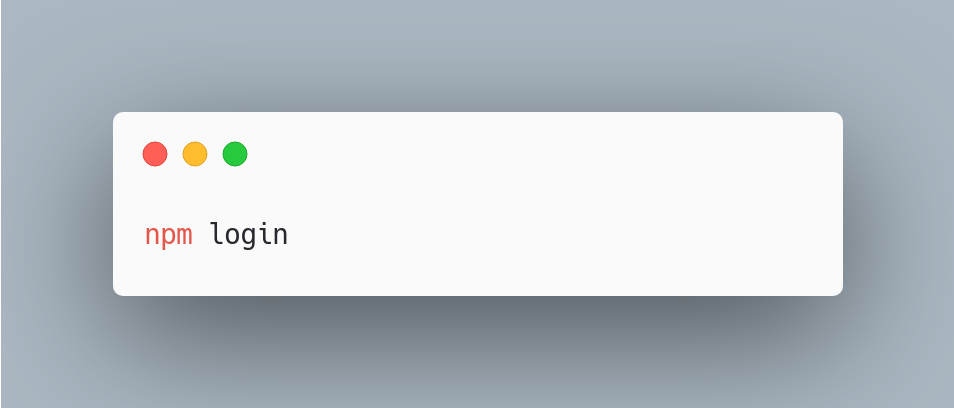
\includegraphics[width=0.7\textwidth]{./Imagenes/8.39.png}
    \caption[ingresar a nuestra cuenta]{Ingresar a nuestra cuenta}
    \end{figure}
    
    Este comando solicitará el nombre de usuario, contraseña y correo electrónico de nuestra cuenta de NPM, es necesario tener una cuenta previamente creada.

Una vez con la sesión iniciada en la terminal es posible publicar nuestro paquete con el siguiente comando.
  \newline
    \begin{figure}[H]
    \centering
    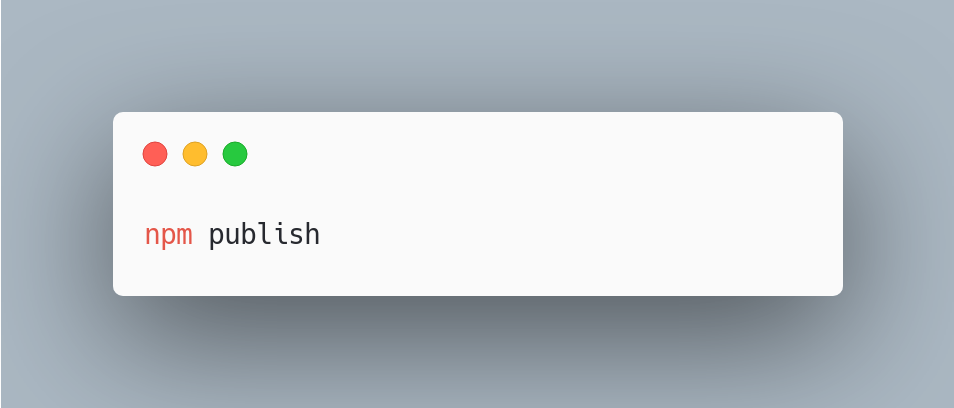
\includegraphics[width=0.7\textwidth]{./Imagenes/8.40.png}
    \caption[Publicar paquete]{Publicar paquete}
    \end{figure}
        Y con esto tenemos nuestra librería publicada.
    \clearpage
    
